\section{Methodology}
\label{sec:methodology}

This section presents the framework (\cref{sec:framework}), the operational model on which all stages are based (\cref{sec:model}), the marginal values of delivered and stored heat and the tariffs derived from them (\cref{sec:derivation}), the response of the local operator and the corrective dispatch (\cref{sec:response}), the reference case and the evaluation metrics (\cref{sec:reference}), and the data and implementation (\cref{sec:data}).

\subsection{Framework}
\label{sec:framework}

The framework mirrors the current setup described in \cref{sec:case_study}: the schedule is set for the whole system, while HTF decides on the discharge into its network according to its own costs. It consists of four stages (\cref{fig:tariff-workflow}).
\begin{enumerate}[label=(\arabic*), leftmargin=*, itemsep=0pt]
    \item \emph{Coordinated schedule.} The operating cost of the upstream system and HTF is minimised jointly. This corresponds to the schedule a system planner would set with perfect information. It provides the PTES charging schedule and the marginal values of delivered and stored heat, and its cost is the lowest cost that any tariff can achieve.
    \item \emph{Tariff derivation.} The marginal values define an hourly discharge credit, which is subtracted from the monthly tariff for discharged heat.
    \item \emph{HTF response.} HTF minimises its own expenditure under the resulting tariff. As in the current setup, HTF is not obliged to follow the discharge schedule; it chooses discharge, heat-exchanger import and heat-pump operation itself, while charging is limited to the scheduled amounts.
    \item \emph{Corrective dispatch.} The upstream units, accumulators and PTES charging are re-dispatched around HTF's decisions, which are kept fixed. This yields the system cost that results from HTF's response.
\end{enumerate}

\begin{figure}[!htb]
    \centering
    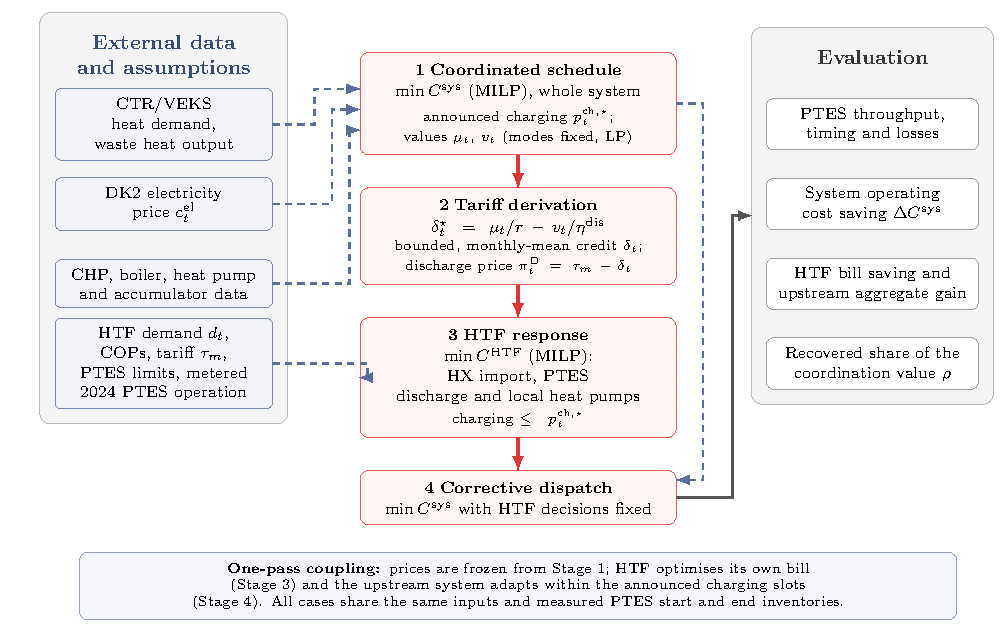
\includegraphics[width=\linewidth]{figures/tariff_workflow.pdf}
    \caption{Framework for deriving and evaluating the PTES discharge tariff. Left: model inputs; dashed arrows indicate which stages use them. Centre: the four stages; solid arrows pass results to the next stage, namely the charging schedule $p^{\mathrm{ch},\star}_t$ and the marginal values $\mu_t$ and $v_t$ from Stage~1, the credit $\delta_t$ and discharge price $\pi^{\mathrm{D}}_t$ from Stage~2, and HTF's decisions from Stage~3. Right: indicators evaluated for each case relative to the measured 2024 operation.}
    \label{fig:tariff-workflow}
\end{figure}

The separation of schedule, response and re-dispatch follows the soft-linking approach of Frigg~\cite{schledorn2022a,schledorn2024frigg}, in which a price-based response is evaluated by a separate model and the dispatch is then solved again with the response fixed. Two properties distinguish the present framework. First, the price is not a decision variable of Stage~1 but is derived from its dual values in Stage~2, and the bounds on the credit (\cref{sec:derivation}) take the role of the bound on the price signal in Frigg. The credit is therefore not necessarily the best one; the cost of Stage~1 and the full-implementation case of \cref{sec:response} bound what any credit could achieve. Second, the responding party is not described by a response function but solves its own optimisation problem. The setting is thus that of a leader who announces a price and a follower who responds, as in bilevel formulations of heat pricing and of incentives between network operators~\cite{bai2022variable,zheng2021incentive}. A bilevel formulation would choose the credit by anticipating HTF's response, which requires HTF's problem, including its binary operating modes, inside the planner's problem. The one-pass scheme uses only information that the planner already has when it sets the schedule, and it corresponds to the order in which a tariff can be applied: the credit is announced with the schedule, HTF responds, and the remaining units adjust. The role of the planner, which schedules the storage while another party operates it, is comparable to electricity market designs in which the system operator manages the state of charge of storage units~\cite{fang2022efficient}.

The stages are run once and are not iterated. Comparing Stages~1 and~4 shows how far a tariff makes the operation that is best for the system also the least-cost operation for HTF. The following assumptions apply to all stages:
\begin{enumerate}[label=(A\arabic*), leftmargin=*, itemsep=0pt]
    \item Demand, electricity prices and waste-heat output are known over the evaluated horizon (perfect foresight).
    \item All units are price takers in the day-ahead electricity market; electricity is bought and sold at the DK2 day-ahead price, also in the corrective dispatch.
    \item The upstream heat system is one node without network constraints; transmission losses are represented by a constant delivery factor.
    \item Payments between companies are transfers and do not enter the system cost.
    \item HTF's response is a rational benchmark, not a behavioural prediction.
\end{enumerate}

\subsection{Operational model}
\label{sec:model}

All stages use the same hourly operational model, a mixed-integer linear programme that combines an economic dispatch of the upstream heat system with a detailed representation of HTF's local system. Models of this type are established for district heating systems with CHP plants and heat storage that sell electricity on the day-ahead market~\cite{rolfsman2004combined,nuytten2013flexibility,fang2016optimization,schledorn2021optimising}. The upstream system comprises the main CHP plants, aggregated waste incineration, peak boilers, regional heat pumps and two heat accumulators. HTF's system comprises the heat-exchanger station, the PTES and two heat pumps (City2 and the Mølleholmen groundwater heat pump); local supply from data-centre surplus heat, other heat recovered from cooling and solar heat is not represented. Powers are hourly averages in MW, and heat flows to HTF and to the PTES are measured as delivered heat. The decisions are collected in two groups: $\mathbf{x}^{\mathrm{up}}$ contains the production, fuel use and electricity output of the upstream units and the operation of the accumulators, and $\mathbf{x}^{\mathrm{loc}}$ contains heat-exchanger import, PTES charging, discharging and inventory, and heat-pump operation.

\subsubsection{Objective}

The coordinated schedule minimises the operating cost of the whole system over the horizon $\mathcal T$,
\begin{subequations}
\label{eq:system}
\begin{equation}
\min_{\mathbf{x}^{\mathrm{up}},\,\mathbf{x}^{\mathrm{loc}}}\; C^{\mathrm{sys}} = \sum_{t\in\mathcal T}\Big[\sum_{u\in\mathcal U}\big(c^{\mathrm{fuel}}_u F_{u,t}+c^{\mathrm{vom}}_u Q_{u,t}\big) + c^{\mathrm{el}}_t\, g^{\mathrm{el}}_t + c^{\mathrm{add}}\, g^{\mathrm{el,heat}}_t + \sum_{i\in\hpset} c^{\mathrm{su},i} z^i_t\Big],
\label{eq:system-cost}
\end{equation}
where $F_{u,t}$ and $Q_{u,t}$ are the fuel input and heat output of upstream unit $u$, $c^{\mathrm{fuel}}_u$ and $c^{\mathrm{vom}}_u$ its fuel price and variable operating cost, and $z^i_t$ indicates a start of heat pump $i$ with start-up cost $c^{\mathrm{su},i}$. The net electricity purchase $g^{\mathrm{el}}_t$ and the electricity used for heat production and pumping, $g^{\mathrm{el,heat}}_t$, are
\begin{align}
g^{\mathrm{el,heat}}_t &= \frac{Q_{\mathrm{eb},t}}{\eta_{\mathrm{eb}}} + \frac{Q_{\mathrm{rhp},t}}{\mathrm{COP}_{\mathrm{rhp}}} + \sum_{i\in\hpset} p^i_t + \kappa\,\big(p^{\mathrm{ch}}_t+p^{\mathrm{dis}}_t\big), \label{eq:el-heat}\\
g^{\mathrm{el}}_t &= g^{\mathrm{el,heat}}_t - \sum_{u\in\mathcal U^{\mathrm{chp}}} P_{u,t} - \sigma_{\mathrm{w}}\,Q_{\mathrm{w},t}, \label{eq:el-balance}
\end{align}
with the electric boiler (eb), the regional heat pumps (rhp), the electricity input $p^i_t$ of HTF's heat pumps, the pumping electricity $\kappa$ per MWh charged or discharged, the electricity output $P_{u,t}$ of the CHP plants and the electricity output of waste incineration in a fixed ratio $\sigma_{\mathrm{w}}$ to its heat output. Electricity is valued at the day-ahead price $c^{\mathrm{el}}_t$ (A2), so $g^{\mathrm{el}}_t$ is negative and reduces the cost when the system is a net seller. Electricity used for heat production and pumping additionally carries the adder $c^{\mathrm{add}}$ for grid tariffs and taxes. National energy and CO$_2$ taxes on fuels are transfers and are not included; fuel prices include the EU ETS allowance cost for fossil fuels.

\subsubsection{Heat balances}

The upstream and the local heat balance are, for all $t\in\mathcal T$,
\begin{align}
& \sum_{u\in\mathcal U} Q_{u,t} + \sum_{a\in\mathcal A}\big(p^{\mathrm{dis}}_{a,t}-p^{\mathrm{ch}}_{a,t}\big) = \frac{D^{\mathrm{reg}}_t - d_t + f^{\mathrm{HX}}_t + p^{\mathrm{ch}}_t}{r} && [\mu_t] \label{eq:upstream-balance}\\
& f^{\mathrm{HX}}_t + p^{\mathrm{dis}}_t + \sum_{i\in\hpset} q^i_t = d_t, \qquad \underline f^{\mathrm{HX}}\le f^{\mathrm{HX}}_t\le \overline f^{\mathrm{HX}}. \label{eq:local-balance}
\end{align}
\Cref{eq:upstream-balance} balances upstream production and the net discharge of the accumulators with the heat that has to be delivered: the regional demand without HTF, $D^{\mathrm{reg}}_t-d_t$, the direct supply to HTF through the heat exchanger, $f^{\mathrm{HX}}_t$, and PTES charging, $p^{\mathrm{ch}}_t$. The delivery factor $r$ accounts for transmission losses (A3). \Cref{eq:local-balance} covers HTF's demand $d_t$ by direct supply, PTES discharge and local heat pumps. The lower limit $\underline f^{\mathrm{HX}}$ keeps the heat-exchanger station in operation. Symbols in brackets denote the dual variables used in \cref{sec:derivation}.

\subsubsection{Upstream units}

The set $\mathcal U$ contains the CHP plants $\mathcal U^{\mathrm{chp}}=\mathcal U^{\mathrm{bp}}\cup\mathcal U^{\mathrm{ex}}$, waste incineration, the peak boilers $\mathcal U^{\mathrm{pb}}$ and the regional heat pumps. The CHP plants are described by their feasible operating region in terms of the power-to-heat ratio $c_{\mathrm{m},u}$ and, for extraction units, the loss of electricity per unit of heat extracted, $c_{\mathrm{v},u}$~\cite{dea2026technologycatalogue,wang2019investigation}. Back-pressure units produce electricity in a fixed ratio to heat and can in addition bypass the turbine to produce heat only,
\begin{align}
& Q_{u,t} = Q^{\mathrm{bp}}_{u,t} + Q^{\mathrm{by}}_{u,t}, \quad P_{u,t} = c_{\mathrm{m},u}\,Q^{\mathrm{bp}}_{u,t}, \quad F_{u,t} = \frac{P_{u,t}}{\eta^{\mathrm{el}}_u} + \frac{Q^{\mathrm{by}}_{u,t}}{\eta^{\mathrm{by}}_u}, && u\in\mathcal U^{\mathrm{bp}}, \label{eq:chp-bp}
\intertext{while extraction units operate between the back-pressure line and condensing operation,}
& F_{u,t} = \frac{P_{u,t} + c_{\mathrm{v},u}\,Q_{u,t}}{\eta^{\mathrm{el}}_u}, \quad P_{u,t} \ge c_{\mathrm{m},u}\,Q_{u,t}, && u\in\mathcal U^{\mathrm{ex}}. \label{eq:chp-ex}
\intertext{Both types are limited by their available electrical, thermal and fuel capacities,}
& P_{u,t}\le \alpha_u\overline P_u, \quad Q_{u,t}\le \alpha_u\big(\overline Q_u+\overline Q^{\mathrm{by}}_u\big), \quad F_{u,t}\le \alpha_u\overline F_u, && u\in\mathcal U^{\mathrm{chp}}, \label{eq:chp-limits}
\end{align}
with availability factor $\alpha_u$ and additional heat capacity in bypass operation $\overline Q^{\mathrm{by}}_u$, which is zero for extraction units. Start-up costs, minimum loads and ramp rates of the CHP plants are not modelled. Waste is incinerated as observed, with heat output $W_t$; only heat in excess of the heat that the system requires in any case, i.e.\ the regional demand without HTF and the minimum flow through the heat exchanger, may be cooled away,
\begin{equation}
\min\big\{W_t,\,(D^{\mathrm{reg}}_t-d_t+\underline f^{\mathrm{HX}})/r\big\} \;\le\; Q_{\mathrm{w},t} \;\le\; W_t. \label{eq:waste}
\end{equation}
Peak boilers and regional heat pumps are limited by their capacities, and the boilers in addition by a common capacity,
\begin{equation}
0\le Q_{u,t}\le \overline Q_u, \quad F_{u,t} = Q_{u,t}/\eta_u, \qquad \sum_{u\in\mathcal U^{\mathrm{pb}}} Q_{u,t} \le \overline Q^{\mathrm{pb}}. \label{eq:boilers}
\end{equation}
The two accumulators $a\in\mathcal A$ are modelled as stores with standing loss $\lambda_a$, a common converter capacity for charging and discharging, and equal inventories at the start and the end of the horizon,
\begin{equation}
e_{a,t} = (1-\lambda_a)\,e_{a,t-1} + p^{\mathrm{ch}}_{a,t} - p^{\mathrm{dis}}_{a,t}, \quad 0\le e_{a,t}\le \overline e_a, \quad p^{\mathrm{ch}}_{a,t}+p^{\mathrm{dis}}_{a,t}\le \overline p_a, \quad e_{a,0}=e_{a,T}=\overline e_a/2. \label{eq:upstream-limits}
\end{equation}

\subsubsection{PTES}

The PTES is represented by its inventory $e_t$ at the end of hour $t$, with standing loss $\lambda$ and charging and discharging efficiencies,
\begin{align}
& e_t = (1-\lambda)\,e_{t-1} + \eta^{\mathrm{ch}} p^{\mathrm{ch}}_t - p^{\mathrm{dis}}_t/\eta^{\mathrm{dis}}, \quad 0\le e_t\le\overline e, \quad e_0=e^{\mathrm{start}},\; e_T=e^{\mathrm{end}} && [v_t] \label{eq:ptes-balance}\\
& \underline p^{k} y^{k}_t \le p^{k}_t \le \overline p^{k} y^{k}_t, \qquad |p^{k}_t-p^{k}_{t-1}|\le r^{\mathrm{PTES}}, \qquad k\in\{\mathrm{ch},\mathrm{dis}\} \label{eq:ptes-limits}\\
& y^{\mathrm{ch}}_t + y^{\mathrm{dis}}_{t'} \le 1,\quad y^{\mathrm{dis}}_t + y^{\mathrm{ch}}_{t'} \le 1, \qquad t'\in\{t,t+1,t+2\}, \qquad y^{\mathrm{ch}}_t,y^{\mathrm{dis}}_t\in\{0,1\}. \label{eq:ptes-modes}
\end{align}
The binary variables $y^{\mathrm{ch}}_t$ and $y^{\mathrm{dis}}_t$ indicate the operating mode. \Cref{eq:ptes-limits} imposes minimum and maximum flows when a mode is active and limits the change in flow between consecutive hours. \Cref{eq:ptes-modes} excludes simultaneous charging and discharging and requires two hours without flow before the direction is reversed. The inventories at the start and the end of the horizon are fixed to the measured inventories at the boundaries of the evaluated period, so that no case can use stored heat without replacing it. Temperatures in the storage are not modelled; the usable capacity $\overline e$ and the flow limits are parameters (\cref{sec:discussion}).

\subsubsection{Local heat pumps}

HTF's heat pumps are modelled as committable units~\cite{taylor2015convex},
\begin{align}
& q^i_t = \mathrm{COP}^i_t\,p^i_t, \qquad \underline\phi\,\overline q^i y^i_t \le q^i_t \le \overline q^i y^i_t, \qquad y^i_t - y^i_{t-1} = z^i_t - w^i_t, \qquad y^i_t,z^i_t,w^i_t\in\{0,1\}, \label{eq:hp}
\end{align}
\end{subequations}
with minimum part load $\underline\phi$, start and stop indicators $z^i_t$ and $w^i_t$, and minimum up and down times of two hours. The coefficients of performance $\mathrm{COP}^i_t$ follow from the ambient temperature and the supply temperature of HTF's network (\cref{app:cop}); start-up costs are taken from~\cite{dea2026technologycatalogue}.

\subsubsection{Coordinated schedule and relation to operational planning}

Stage~1 solves problem~\eqref{eq:system}, that is, it minimises \cref{eq:system-cost} subject to \cref{eq:el-heat,eq:el-balance,eq:upstream-balance,eq:local-balance,eq:chp-bp,eq:chp-ex,eq:chp-limits,eq:waste,eq:boilers,eq:upstream-limits,eq:ptes-balance,eq:ptes-limits,eq:ptes-modes,eq:hp}. Its solution is denoted by a star; in particular, $p^{\mathrm{ch},\star}_t$ and $p^{\mathrm{dis},\star}_t$ are the coordinated charging and discharging schedules and $C^{\mathrm{sys}}_{\mathrm{coord}}$ is the minimal system cost.

The coordinated schedule follows the same principle as Varmelast's dispatch (\cref{sec:case_study}): units are used in the order of their heat production cost, i.e.\ their variable fuel and operating cost net of the electricity revenue of CHP units, and storage shifts production from expensive to cheap hours. In \cref{eq:system-cost}, the electricity revenue enters through the net electricity purchase $g^{\mathrm{el}}_t$; a back-pressure unit therefore has a low or negative net heat production cost when electricity prices are high. Minimising \cref{eq:system-cost} over all hours jointly yields this merit order in every hour and, in addition, the use of the accumulators and the PTES. The model differs from operational planning by assumptions (A1)--(A3) and by constant fuel prices.

\subsection{Marginal values and discharge credit}
\label{sec:derivation}

\subsubsection{Marginal values of delivered and stored heat}

Problem~\eqref{eq:system} contains binary variables, so its dual variables are not defined. Following the approach of \citet{oneill2005efficient} for markets with non-convexities, all binary variables are fixed at their optimal values and the problem is solved again as a linear programme, whose dual variables can be interpreted as prices. They are marginal values conditional on the operating modes: they do not include the cost of changing a mode. Two of them are used. The dual variable $\mu_t$ of the upstream balance~\eqref{eq:upstream-balance} is the marginal heat cost of the system, i.e.\ the net production cost of the last unit used in the merit order of hour $t$, or the value that storage assigns to heat in that hour if a store is at its limit. One additional MWh delivered to HTF costs $\mu_t/r$. The dual variable $v_t$ of the storage balance~\eqref{eq:ptes-balance} is the value of one additional MWh in the PTES at the end of hour $t$; it reflects the marginal heat cost of the hours in which the stored heat is expected to be used. Neither value is a settlement price: the heat is billed at the monthly tariff (\cref{sec:case_study}).

\subsubsection{Value spread}

Consider replacing one MWh of direct supply by discharge in hour $t$. For the system, this saves $\mu_t/r$ of upstream production, uses stored heat worth $v_t/\eta^{\mathrm{dis}}$ and requires pumping electricity costing $\kappa\,(c^{\mathrm{el}}_t+c^{\mathrm{add}})$. For HTF, which pays the tariff $\tau_m$ for direct heat and $\tau_m-\delta_t$ for discharged heat, the same substitution saves the credit $\delta_t$ and requires the same pumping. The marginal incentive of HTF equals the marginal value for the system if
\begin{equation}
\delta^{\star}_t = \frac{\mu_t}{r} - \frac{v_t}{\eta^{\mathrm{dis}}},
\label{eq:value-spread}
\end{equation}
that is, if the credit equals the value of delivering heat now rather than keeping it stored. This \emph{value spread} differs from the marginal cost of heat used in dynamic heat pricing~\cite{dominkovic2018influence,liu2019marginal}: it is the difference between two marginal values, which arises because the storage links the hours of the horizon.

The optimality conditions of the linear programme show how the spread relates to the schedule. In hours in which the heat exchanger is not at a limit, the net value $\delta^{\star}_t-\kappa\,(c^{\mathrm{el}}_t+c^{\mathrm{add}})$ equals the net multiplier of the flow and ramp limits on discharge in hour $t$. It is zero when the scheduled discharge lies strictly within these limits, and positive when the schedule is at the maximum discharge, i.e.\ when the system would benefit from more discharge than is feasible. In discharge hours, the spread therefore exceeds the pumping cost only by the scarcity value of the discharge limits. In hours without discharge, the spread is conditional on the operating mode: it is usually below the pumping cost, but it can exceed it where the operating rules, such as the minimum flow or the lock-out after charging, prevent a discharge that would otherwise be worthwhile. The alignment in \cref{eq:value-spread} is a marginal one. HTF's own constraints on inventory, flows and operating modes add scarcity values on its side, and the dual values need not be unique. Whether a credit based on the spread leads HTF to the coordinated discharge is therefore tested by optimising HTF's response (\cref{sec:response}) and is not assumed.

\subsubsection{Tariff design}

All tariffs keep the monthly tariff $\tau_m$ for direct heat and differ only in the credit on discharged heat, so that the discharge price is $\pi^{\mathrm{D}}_t=\tau_m-\delta_t$. Three credits are derived, which differ in what they take from the value spread (\cref{tab:cases}).

The \emph{bounded credit}, referred to as the hourly credit, keeps the timing of $\delta^{\star}_t$ and fixes its level,
\begin{equation}
\delta_t = \min\Big\{\max\big\{a_m + g\,(\delta^{\star}_t-\overline{\delta^{\star}}_m),\,0\big\},\,\overline\delta\Big\},
\qquad \frac{1}{|\mathcal T_m|}\sum_{t\in\mathcal T_m}\delta_t = \delta^{\mathrm{mean}},
\label{eq:bounded-credit}
\end{equation}
where $\overline{\delta^{\star}}_m$ is the mean spread over the hours $\mathcal T_m$ of month $m$, $g$ the strength with which the credit follows the spread, $\overline\delta$ the upper bound, and the intercept $a_m$ is determined for each month such that the mean credit equals $\delta^{\mathrm{mean}}$. The base case uses $g=0.25$, $\overline\delta=10$~DKK/MWh and $\delta^{\mathrm{mean}}=5$~DKK/MWh. The credit pays more in hours in which discharge is more valuable than on average in the month, but its level is set by design, so the payment to HTF is small and predictable. The bounds limit the transfer in the same way as the bound on the price signal limits the welfare loss of consumers in Frigg~\cite{schledorn2024frigg}.

The \emph{value share} passes a share $s$ of the positive spread to HTF,
\begin{equation}
\delta_t = s\,\max\{\delta^{\star}_t,0\},\qquad s\in\{0.25,\,0.5,\,1\}.
\label{eq:shared-credit}
\end{equation}
It uses both the timing and the level of the spread: HTF receives a fixed fraction of the value of discharging, so the payment grows with the value and with $s$, similar to sharing a profit.

A \emph{constant credit} of 5~DKK/MWh, with the same mean as \cref{eq:bounded-credit}, ignores the spread and isolates the effect of timing.

\begin{table}[!htb]
    \centering
    \small
    \caption{Evaluated cases. All tariff cases keep the monthly tariff for direct heat and differ only in the credit on discharged heat.}
    \label{tab:cases}
    \begin{tabular}{p{0.24\linewidth}p{0.30\linewidth}p{0.36\linewidth}}
        \toprule
        Case & Credit on discharged heat & Interpretation \\
        \midrule
        Measured 2024 (reference) & none & Current settlement; PTES flows as metered \\
        Coordinated schedule & -- & Lowest system cost; upper bound for any tariff \\
        Constant credit & 5~DKK/MWh in every hour & Same payment level as the hourly credit, without timing \\
        Hourly credit & \cref{eq:bounded-credit}; 0--10~DKK/MWh, mean 5 & Timing of the storage value, fixed payment level \\
        Value share $s$ & \cref{eq:shared-credit}; share $s$ of the storage value & Timing and level of the storage value; payment grows with $s$ \\
        Schedule followed & none or hourly credit & PTES fixed to the coordinated schedule (\cref{sec:results-implementation}) \\
        \bottomrule
    \end{tabular}
\end{table}

\subsection{HTF response and corrective dispatch}
\label{sec:response}

\subsubsection{HTF response}

In Stage~3, HTF minimises its expenditure for a given credit. Charging heat and the pumping electricity for charging remain with the upstream side, so HTF's expenditure consists of its heat payments and of the electricity and start-up costs of its own operation,
\begin{equation}
\min_{\mathbf{x}^{\mathrm{loc}}}\; C^{\mathrm{HTF}} = \sum_{t\in\mathcal T}\Big[\underbrace{\tau_m f^{\mathrm{HX}}_t + (\tau_m-\delta_t)\,p^{\mathrm{dis}}_t}_{\text{heat payment}} + \underbrace{\big(c^{\mathrm{el}}_t+c^{\mathrm{add}}\big)\Big(\sum_{i\in\hpset} p^i_t + \kappa\,p^{\mathrm{dis}}_t\Big) + \sum_{i\in\hpset} c^{\mathrm{su},i} z^i_t}_{\text{own operating cost}}\Big]
\label{eq:htf-cost}
\end{equation}
subject to the local balance~\eqref{eq:local-balance}, the PTES constraints~\eqref{eq:ptes-balance}--\eqref{eq:ptes-modes}, the heat-pump constraints~\eqref{eq:hp} and
\begin{equation}
0\le p^{\mathrm{ch}}_t\le p^{\mathrm{ch},\star}_t \qquad \forall t\in\mathcal T.
\label{eq:charging-limit}
\end{equation}
HTF thus decides on heat-exchanger import, discharge and local heat-pump operation, while charging is limited to the scheduled amounts. The schedule enters HTF's problem only through this limit and through the credit derived from it; the PTES inventory at the end of the horizon is the same as in the coordinated schedule. Whether HTF's discharge coincides with the schedule is therefore a result of the tariff, not an assumption. This corresponds to self-scheduling in response to a published price signal, as opposed to participation in the central dispatch~\cite{frolke2022market}.

In the \emph{full-implementation} case, $p^{\mathrm{ch}}_t$ and $p^{\mathrm{dis}}_t$ are additionally fixed to the coordinated schedule, and HTF chooses only heat-exchanger import and heat-pump operation. It shows the outcome if the schedule were implemented exactly under a given settlement.

\subsubsection{Corrective dispatch}

Stage~4 determines how the upstream system adjusts to HTF's decisions. It solves problem~\eqref{eq:system} with $f^{\mathrm{HX}}_t$, $p^{\mathrm{dis}}_t$ and $q^i_t$ fixed to HTF's response and with the charging limit~\eqref{eq:charging-limit}. Only the upstream units, the accumulators and PTES charging are adjusted; HTF's decisions are not revised. The resulting cost $C^{\mathrm{sys}}_k$ is the system operating cost of case $k$. Because electricity is valued at the day-ahead price also in this stage (A2), the cost of deviating from an electricity position that was sold before the deviation became known is not included.

\subsection{Reference case and evaluation}
\label{sec:reference}

\subsubsection{Reference case}

The reference is the measured 2024 operation. PTES charging and discharging are fixed to the metered hourly flows, without the design limits of \cref{eq:ptes-limits,eq:ptes-modes}; HTF's heat-exchanger import and heat pumps follow \cref{eq:htf-cost} with $\delta_t=0$, and the upstream system is re-dispatched as in Stage~4. With the modelled standing loss, the replayed inventory ends the year 27~MWh above the measured inventory, with a mean absolute deviation of 73~MWh; remaining differences at the end of a period are valued at the final value of stored heat from Stage~1.

\subsubsection{Evaluation metrics}

Three accounts are distinguished for each case $k$. The system operating cost $C^{\mathrm{sys}}_k$ results from Stage~4. HTF's expenditure $B^{\mathrm{HTF}}_k$ is the value of \cref{eq:htf-cost} and consists of the heat payment $R_k$ and HTF's own operating cost $C^{\mathrm{loc}}_k$. The upstream side is treated as one aggregate account, whose surplus is the heat payment received less the upstream operating cost, $U_k = R_k - (C^{\mathrm{sys}}_k - C^{\mathrm{loc}}_k)$. Each tariff is evaluated by the changes relative to the reference,
\begin{equation}
\Delta C^{\mathrm{sys}} = C^{\mathrm{sys}}_{\mathrm{ref}}-C^{\mathrm{sys}}_k, \qquad
\Delta B^{\mathrm{HTF}} = B^{\mathrm{HTF}}_{\mathrm{ref}}-B^{\mathrm{HTF}}_k, \qquad
\Delta U = U_k-U_{\mathrm{ref}},
\end{equation}
which satisfy the identity
\begin{equation}
\Delta C^{\mathrm{sys}} = \Delta B^{\mathrm{HTF}} + \Delta U, \qquad
\rho = \frac{\Delta C^{\mathrm{sys}}}{C^{\mathrm{sys}}_{\mathrm{ref}}-C^{\mathrm{sys}}_{\mathrm{coord}}}.
\label{eq:evaluation}
\end{equation}
The heat payment cancels in the sum, so a tariff increases welfare only if $\Delta C^{\mathrm{sys}}>0$, and it is acceptable to both sides only if $\Delta B^{\mathrm{HTF}}\ge0$ and $\Delta U\ge0$. The denominator of $\rho$ is the \emph{coordination value}, the cost difference between the reference and the coordinated schedule, and $\rho$ is the share of it that a tariff recovers. $\Delta U$ combines VEKS and the producers; its allocation between them depends on the heat purchase agreements and is not resolved here. In addition, the PTES discharge and the equivalent full cycles, i.e.\ the discharge divided by the capacity $\overline e$, are reported. When counting the weeks in which both sides gain, the sum of the absolute optimality gaps of the problems compared is used as tolerance.

\subsection{Data, parameters and implementation}
\label{sec:data}

Hourly CTR and VEKS demand, production by technology and waste output for 2024 are taken from Varmelast, and DK2 prices from Energi Data Service. Metered PTES flows and the temperature-based inventory come from the monitoring data of the storage~\cite{sifnaios2025performance}. Plant parameters follow the FFH50 planning assumptions; fuel prices and availability factors are scenario values (\cref{app:units}). The gas price of 350~DKK/MWh corresponds approximately to the 2024 TTF average plus the EU ETS allowance cost; biomass is zero-rated in the EU ETS. HTF's hourly demand is a 2019 profile mapped to 2024 (348~GWh); its peak of 98.9~MW lies below the limit of the heat-exchanger station, which is therefore not binding in any hour. \Cref{tab:parameters} lists the main parameters.

The year is evaluated as 52 weekly horizons; each starts and ends at the measured PTES inventory, so that the weekly results can be summed. The model is implemented in PyPSA~\cite{brown2018pypsa} with additional Linopy constraints for the operating rules of the PTES and the heat pumps. Mixed-integer problems are solved to a relative gap of $10^{-4}$, and HTF's problems to $10^{-8}$, because the differences in HTF's expenditure between tariffs are small.

\begin{table}[!htb]
    \centering
    \small
    \caption{Main parameters. $^{\dagger}$Provisional assumption.}
    \label{tab:parameters}
    \begin{tabular}{lll}
        \toprule
        Parameter & Value & Note \\
        \midrule
        PTES capacity $\overline e$ & 3,300 MWh & \\
        Charge / discharge limits $\overline p^{\mathrm{ch}},\overline p^{\mathrm{dis}}$ & 30 / 30 MW & Minimum 10 / 5 MW when active \\
        Ramp limit $r^{\mathrm{PTES}}$ & 12 MW/h & \\
        Standing loss $\lambda$ & 0.0275\,\%/h & Consistent with metered 2024 losses \\
        Efficiencies $\eta^{\mathrm{ch}},\eta^{\mathrm{dis}}$ & 1 / 1 & Losses represented by $\lambda$ \\
        Pumping electricity $\kappa$ & 0.005 MWh/MWh$^{\dagger}$ & Per MWh charged and discharged \\
        Heat exchanger $\underline f^{\mathrm{HX}},\overline f^{\mathrm{HX}}$ & 0.5 / 100 MW & Station towards HTF \\
        Heat pumps $\overline q^{\mathrm{c2}},\overline q^{\mathrm{gw}}$ & 1.34 / 1.50 MW & COP 3.1--3.6 / 3.0--3.3; $\underline\phi=0.25$ \\
        Electricity adder $c^{\mathrm{add}}$ & 125 DKK/MWh$^{\dagger}$ & Grid tariffs and taxes \\
        Delivery factor $r$ & 0.98$^{\dagger}$ & Transmission losses \\
        Monthly tariff $\tau_m$ & 153--387 DKK/MWh & 2024 \\
        CHP (AMV1, AMV4, AVV1, AVV2, KKV8) & 1,521 MW & Heat capacity, 90\% availability (\cref{tab:units}) \\
        Waste incineration & 519.5 MW & Observed 2024 output; $\sigma_{\mathrm{w}}=0.25$ \\
        Peak boilers / regional heat pumps & 2,033 / 20 MW & \\
        Accumulators (AMV / AVV) & 1,000 / 2,200 MWh & 300 / 330 MW; $\lambda_a=0.01$\,\%/h \\
        \bottomrule
    \end{tabular}
\end{table}
